\documentclass[aspectratio=169]{beamer}

\usetheme{Madrid}
\usecolortheme{beaver}
\usepackage[spanish]{babel}
\usepackage[utf8]{inputenc}
\usepackage{amsmath}
\usepackage{amssymb}
\usepackage{booktabs}
\usepackage{xcolor}
\usepackage{tikz}
\usepackage{graphicx}

\definecolor{primaryblue}{RGB}{31, 73, 125}
\definecolor{accentorange}{RGB}{204, 102, 0}

\setbeamercolor{frametitle}{bg=primaryblue, fg=white}
\setbeamercolor{title}{bg=primaryblue, fg=white}
\setbeamercolor{structure}{fg=primaryblue}
\setbeamercolor{block title}{bg=primaryblue, fg=white}
\setbeamercolor{alerted text}{fg=accentorange}

\title[Optimización en Finanzas]{Algoritmos Bioinspirados Aplicados a Finanzas}
\subtitle{Diversidad de Carteras con AEs y Optimización con PSO}
\author{Óscar Vera López}
\institute{Trabajo de Computación Bioinspirada - Máster en Inteligencia Artificial}
\date{Junio 2026}

\setbeamertemplate{navigation symbols}{}
\setbeamertemplate{footline}[frame number]

\begin{document}

% =========================================================
%  PORTADA
% =========================================================
\begin{frame}
  \titlepage
\end{frame}

% =========================================================
%  ÍNDICE GENERAL
% =========================================================
\begin{frame}{Índice}
  \tableofcontents
\end{frame}

% =========================================================
%  PARTE 1
% =========================================================
\section{Parte 1: Problema de Máxima Diversidad}

% --- Motivación ------------------------------------------
\begin{frame}{Contexto y Motivación}
  \begin{columns}[T]
    \begin{column}{0.55\textwidth}
      \textbf{Objetivo financiero}\\[6pt]
      Construir una cartera de exactamente $m$ acciones del S\&P 500
      que \alert{maximice la descorrelación} entre activos, reduciendo teóricamente
      así el riesgo ante caídas del mercado.

      \vspace{10pt}
      \textbf{Adaptación del problema de máxima diversidad}
      \begin{itemize}
        \item El problema original maximiza la diversidad geométrica.
        \item Aquí la \emph{distancia} entre dos acciones $i,j$ es
              $d_{ij} = 1 - \rho_{ij}$ (correlación de Pearson).
        \item Minimizar $-\sum d_{ij}x_ix_j$ equivale a maximizar la
              descorrelación total de la cartera.
      \end{itemize}
    \end{column}
    \begin{column}{0.42\textwidth}
      \begin{block}{Datos utilizados}
        \begin{itemize}
          \item \textbf{Universo:} hasta 200 empresas del S\&P 500
          \item \textbf{Periodo:} 2014-2020 (precios diarios)
          \item \textbf{Entrenamiento:} 2014-2018
          \item \textbf{Test (backtest):} 2019-2020
          \item \textbf{Fuente:} Yahoo Finance vía \texttt{yfinance}
        \end{itemize}
      \end{block}
    \end{column}
  \end{columns}
\end{frame}

% --- Formulación -----------------------------------------
\begin{frame}{Formulación Matemática}
  \textbf{Variables de decisión:} $x_i \in \{0,1\}$, $i = 1,\ldots,n$
  \quad ($x_i = 1$ si se incluye la acción $i$ en la cartera)
  \textbf{Función objetivo a minimizar:}
  \[
    F(\mathbf{x}) =
    \begin{cases}
      -\displaystyle\sum_{i=1}^{n-1}\sum_{j=i+1}^{n} d_{ij}\,x_i\,x_j
        & \text{si } \displaystyle\sum_{i=1}^{n} x_i = m \\[10pt]
      \displaystyle\left|\sum_{i=1}^{n} x_i - m\right|
        & \text{en otro caso}
    \end{cases}
  \]

  \vspace{8pt}
  \begin{columns}[T]
    \begin{column}{0.48\textwidth}
      \begin{alertblock}{Observaciones clave}
        \begin{itemize}
          \item Soluciones \emph{factibles} tienen $F < 0$.
          \item Soluciones \emph{no factibles} tienen $F > 0$.
          \item El AE aprende a descartar no factibles porque su
                fitness es siempre peor.
        \end{itemize}
      \end{alertblock}
    \end{column}
    \begin{column}{0.48\textwidth}
      \begin{block}{Matriz de distancias}
        $d_{ij} = 1 - \rho_{ij}$\\[4pt]
        $\rho_{ij}$ = correlación de Pearson de los retornos diarios
        entre la acción $i$ y la acción $j$ durante el periodo de
        entrenamiento.
      \end{block}
    \end{column}
  \end{columns}
\end{frame}

% --- AE general ------------------------------------------
\begin{frame}{Algoritmo Evolutivo Base}
  \begin{columns}[T]
    \begin{column}{0.48\textwidth}
      \textbf{Representación}
      \begin{itemize}
        \item Cromosoma binario de longitud $n$.
        \item Gen $i = 1 \Rightarrow$ acción $i$ en cartera.
      \end{itemize}
      \textbf{Selección}
      \begin{itemize}
        \item Torneo de tamaño $k = 3$ (minimización).
      \end{itemize}
      \textbf{Cruce}
      \begin{itemize}
        \item Cruce uniforme, $p_c = 0{,}6$.
      \end{itemize}
      \textbf{Mutación}
      \begin{itemize}
        \item Flip-bit con $p_m = 1/n$.
      \end{itemize}
      \textbf{Elitismo}
      \begin{itemize}
        \item Mejor individuo histórico pasa intacto.
      \end{itemize}
    \end{column}
    \begin{column}{0.48\textwidth}
      \begin{block}{Dos enfoques para gestionar restricciones}
        \vspace{4pt}
        \textbf{AE1 - Penalización}\\
        Si $\|\mathbf{x}\|_1 \neq m$, sustituye la diversidad
        por una penalización positiva.
        Permite explorar soluciones no factibles.
        \\
        \vspace{8pt}
        \textbf{AE2 - Reparación}\\
        Antes de evaluar, ajusta el cromosoma para que
        tenga exactamente $m$ unos.
        Siempre evalúa soluciones factibles.
      \end{block}

      \vspace{8pt}
      \begin{block}{Parámetros comunes}
        Pop.\ = 50 \quad Gen.\ = 150 \quad Runs = 10
      \end{block}
    \end{column}
  \end{columns}
\end{frame}

% --- AE1 -------------------------------------------------
\begin{frame}{AE1: Penalización vs.\ AE2: Reparación}
  \begin{columns}[T]
    \begin{column}{0.48\textwidth}
      \begin{block}{AE1: Penalización}
        \[
          F_{\text{AE1}}(\mathbf{x}) =
          \begin{cases}
            -\sum d_{ij}x_ix_j & \|\mathbf{x}\|_1 = m\\
            \bigl|\|\mathbf{x}\|_1 - m\bigr| & \text{si no}
          \end{cases}
        \]
        \begin{itemize}
          \item Mayor exploración del espacio.
          \item El AE aprende a evitar violaciones por sí solo.
        \end{itemize}
      \end{block}
    \end{column}
    \begin{column}{0.48\textwidth}
      \begin{block}{AE2: Algoritmo de Reparación}
        \begin{enumerate}
          \item Si $k > m$: eliminar $k-m$ unos aleatorios.
          \item Si $k < m$: añadir $m-k$ unos aleatorios.
          \item Evaluar el cromosoma reparado.
        \end{enumerate}
        \begin{itemize}
          \item Búsqueda siempre dentro del espacio factible.
          \item Convergencia más estable y reproducible.
        \end{itemize}
      \end{block}
    \end{column}
  \end{columns}

  \vspace{8pt}
  \begin{columns}[T]
    \begin{column}{0.48\textwidth}
      \begin{alertblock}{Analogía AE1}
        Gestor que \emph{penaliza} carteras ilegales,
        pero las evalúa igualmente.
      \end{alertblock}
    \end{column}
    \begin{column}{0.48\textwidth}
      \begin{alertblock}{Analogía AE2}
        Bróker que \emph{rebalancea} antes de presentar
        la cartera al comité de inversión.
      \end{alertblock}
    \end{column}
  \end{columns}
\end{frame}

% --- Escenarios de prueba --------------------------------
\begin{frame}{Diseño Experimental: Stress Test}
  \begin{columns}[T]
    \begin{column}{0.5\textwidth}
      \textbf{Tres escenarios de inversión}\\[6pt]
      \begin{tabular}{lcc}
        \toprule
        Escenario & $n$ & $m$ \\
        \midrule
        Cartera Pequeña      & 100 & 10 \\
        Cartera Mediana      & 150 & 15 \\
        Cartera Institucional & 200 & 20 \\
        \bottomrule
      \end{tabular}

      \vspace{10pt}
      \textbf{Protocolo estadístico}
      \begin{itemize}
        \item 10 ejecuciones por escenario y enfoque.
        \item Semillas fijas (0-9) para reproducibilidad.
        \item Test no paramétrico de Wilcoxon para comparar
              AE1 vs AE2 ($p < 0{,}05$).
      \end{itemize}
    \end{column}
    \begin{column}{0.47\textwidth}
      \begin{block}{¿Por qué Wilcoxon?}
        \begin{itemize}
          \item No asume normalidad de los resultados.
          \item Apropiado para muestras pequeñas ($n=10$).
          \item Evalúa si las diferencias entre pares de
                resultados son sistemáticas o debidas al azar.
        \end{itemize}
      \end{block}

      \vspace{8pt}
      \begin{alertblock}{Espacio de búsqueda}
        Cartera Institucional: $\binom{200}{20} \approx 10^{26}$
        combinaciones posibles.
        El AE solo evalúa $50 \times 150 = 7500$ individuos
        por run.
      \end{alertblock}
    \end{column}
  \end{columns}
\end{frame}

% --- Resultados estadísticos ----------------------------
\begin{frame}{Resultados Estadísticos}
  \begin{columns}[T]
    \begin{column}{0.48\textwidth}
      \textbf{Diversidad media obtenida (10 runs)}\\[4pt]
      \begin{tabular}{lccc}
        \toprule
        Escenario & AE1 & AE2 & $p$-value \\
        \midrule
        Pequeña       & 40.74 & \textbf{41.13} & 0.0020* \\
        Mediana       & 91.68 & \textbf{93.87} & 0.0020* \\
        Institucional & 162.49 & \textbf{167.40} & 0.0020* \\
        \bottomrule
      \end{tabular}
      {\footnotesize * diferencia estadísticamente significativa ($p<0{,}05$)}

      \vspace{8pt}
      \begin{tabular}{lcc}
        \toprule
        Algoritmo & Victorias & Sig.\ \\
        \midrule
        AE1 (Penalización) & 0/3 & 0 \\
        AE2 (Reparación)   & 3/3 & 3 \\
        \bottomrule
      \end{tabular}
    \end{column}
    \begin{column}{0.48\textwidth}
      \begin{alertblock}{Conclusión principal}
        AE2 (reparación) supera a AE1 en los tres escenarios,
        con diferencias significativas en todos ($p=0{,}0020$).
      \end{alertblock}
      \begin{block}{Interpretación}
        La reparación restringe la búsqueda al espacio factible
        desde el inicio: converge a mayor diversidad y con mucha
        menor varianza entre runs (std $0{,}04$--$0{,}14$ frente a
        $0{,}17$--$1{,}23$ de la penalización). La penalización
        malgasta evaluaciones escapando de soluciones no factibles.
      \end{block}
    \end{column}
  \end{columns}
\end{frame}

% --- Curvas de convergencia - con imagen -----------------
\begin{frame}{Curvas de Convergencia (10 runs por escenario)}
  \begin{columns}[T]
    \begin{column}{0.38\textwidth}
      \textbf{Lo que muestran las curvas}
      \begin{itemize}
        \item \textcolor{primaryblue}{\textbf{Azul (AE1):}} arranca
              muy bajo (la población inicial casi nunca es factible),
              trepa al entrar en la región factible y se queda en
              diversidad algo menor, con más varianza entre runs.
        \item \textcolor{accentorange}{\textbf{Naranja (AE2):}}
              factible desde el inicio; converge suave a la
              \alert{mayor diversidad} y casi sin dispersión.
        \item Resultado consistente en los tres tamaños:
              la reparación domina a la penalización.
      \end{itemize}
    \end{column}
    \begin{column}{0.60\textwidth}
      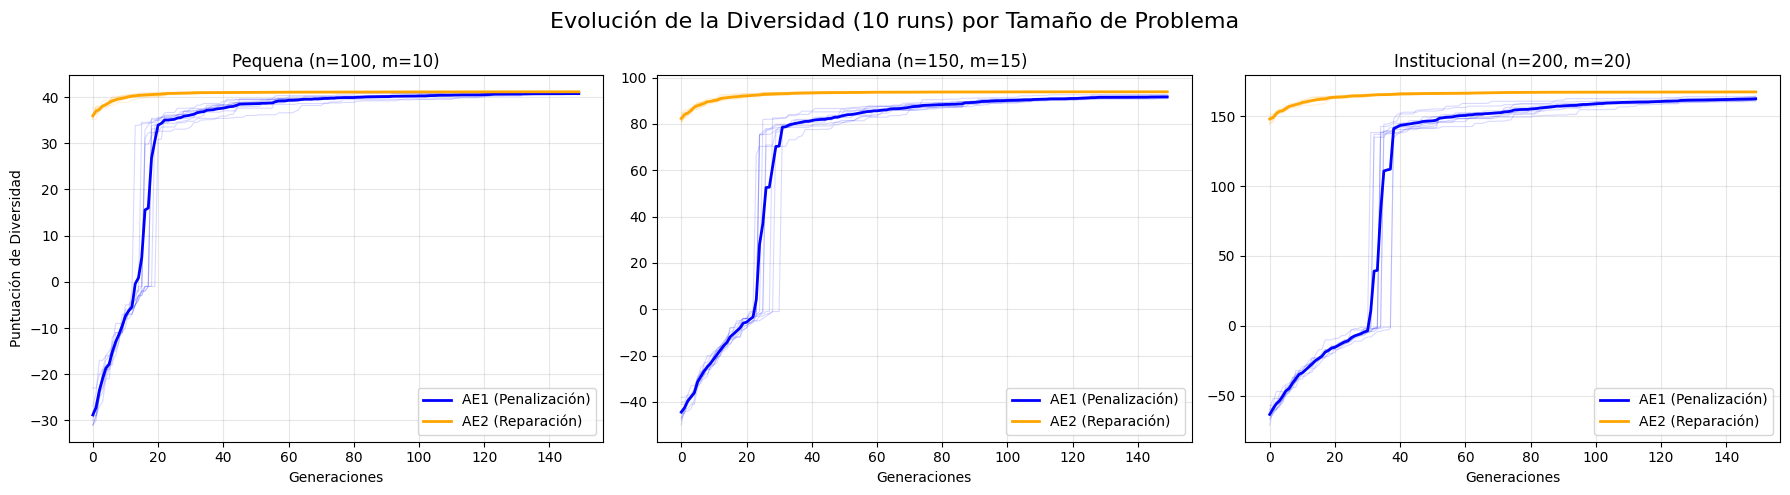
\includegraphics[width=\linewidth, clip=true, trim=865 0 0 30]{img/corr_convergencia.png}
    \end{column}
  \end{columns}
\end{frame}

% --- Backtest - metodología ------------------------------
\begin{frame}{Backtest Financiero - Metodología (2019-2020)}
  \begin{columns}[T]
    \begin{column}{0.5\textwidth}
      \textbf{Protocolo out-of-sample}
      \begin{itemize}
        \item Se toma el \emph{mejor run} de cada enfoque.
        \item Cartera equiponderada con las $m$ acciones
              seleccionadas \emph{solo con datos hasta 2018}.
        \item Se evalúa en el periodo 2019-2020 (nunca visto).
        \item Benchmark: media equiponderada de los $n$ activos.
      \end{itemize}

      \vspace{8pt}
      \textbf{Tres métricas complementarias}
      \begin{itemize}
        \item \textbf{Retorno acumulado} - rentabilidad bruta.
        \item \textbf{Drawdown} - caída máxima desde el pico.
        \item \textbf{Volatilidad móvil 30d} - riesgo dinámico.
      \end{itemize}
    \end{column}
    \begin{column}{0.47\textwidth}
      \begin{alertblock}{Limitación fundamental}
        Maximizar la descorrelación \emph{no} implica minimizar
        el riesgo de pérdidas absolutas.

        \vspace{4pt}
        Concentrar la cartera en solo $m$ activos sacrifica la
        diversificación que aporta el \emph{número} de posiciones
        y eleva el riesgo idiosincrático.
      \end{alertblock}

      \vspace{6pt}
      \begin{block}{Hipótesis a validar}
        Cartera de máxima descorrelación $\Rightarrow$ ¿menor
        volatilidad y drawdown que el benchmark amplio?
      \end{block}
    \end{column}
  \end{columns}
\end{frame}

% --- Backtest - cartera institucional -------------------
\begin{frame}{Backtest}
  \begin{columns}[T]
    \begin{column}{0.5\textwidth}
       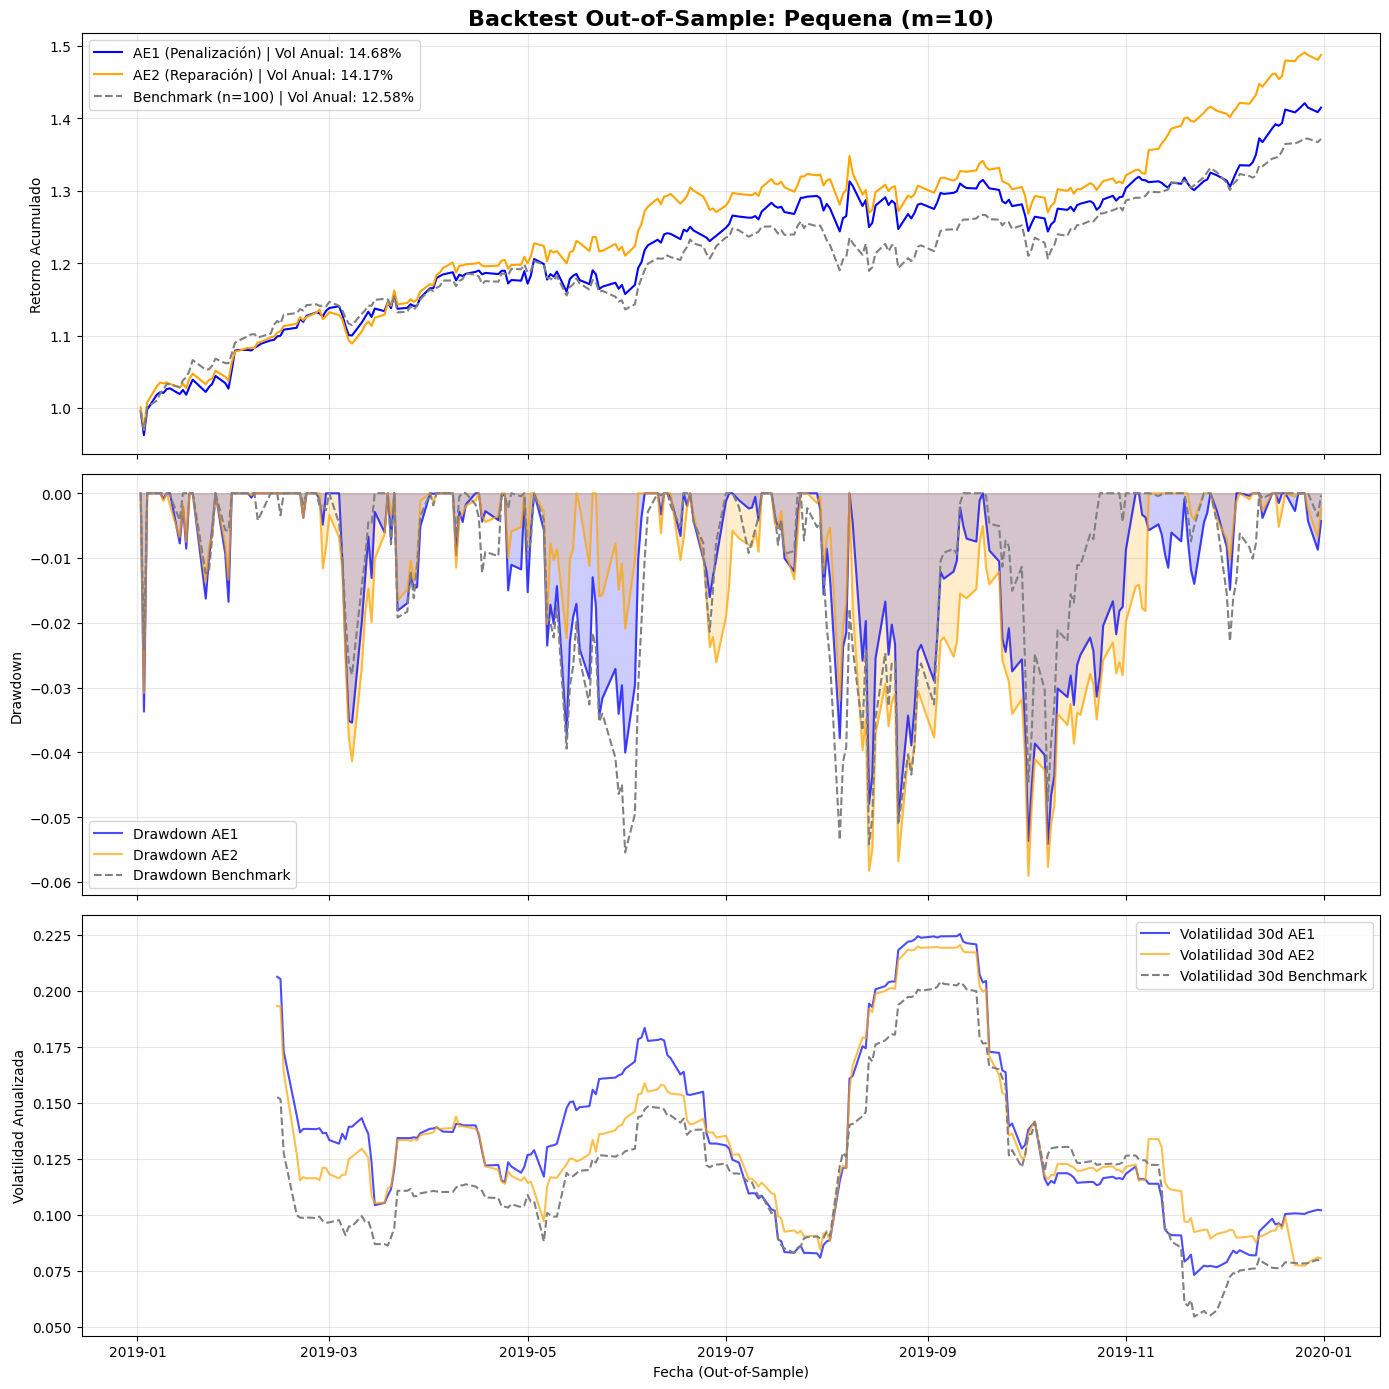
\includegraphics[width=\linewidth]{img/corr_backtest_pequena.png}
    \end{column}
    \begin{column}{0.5\textwidth}
      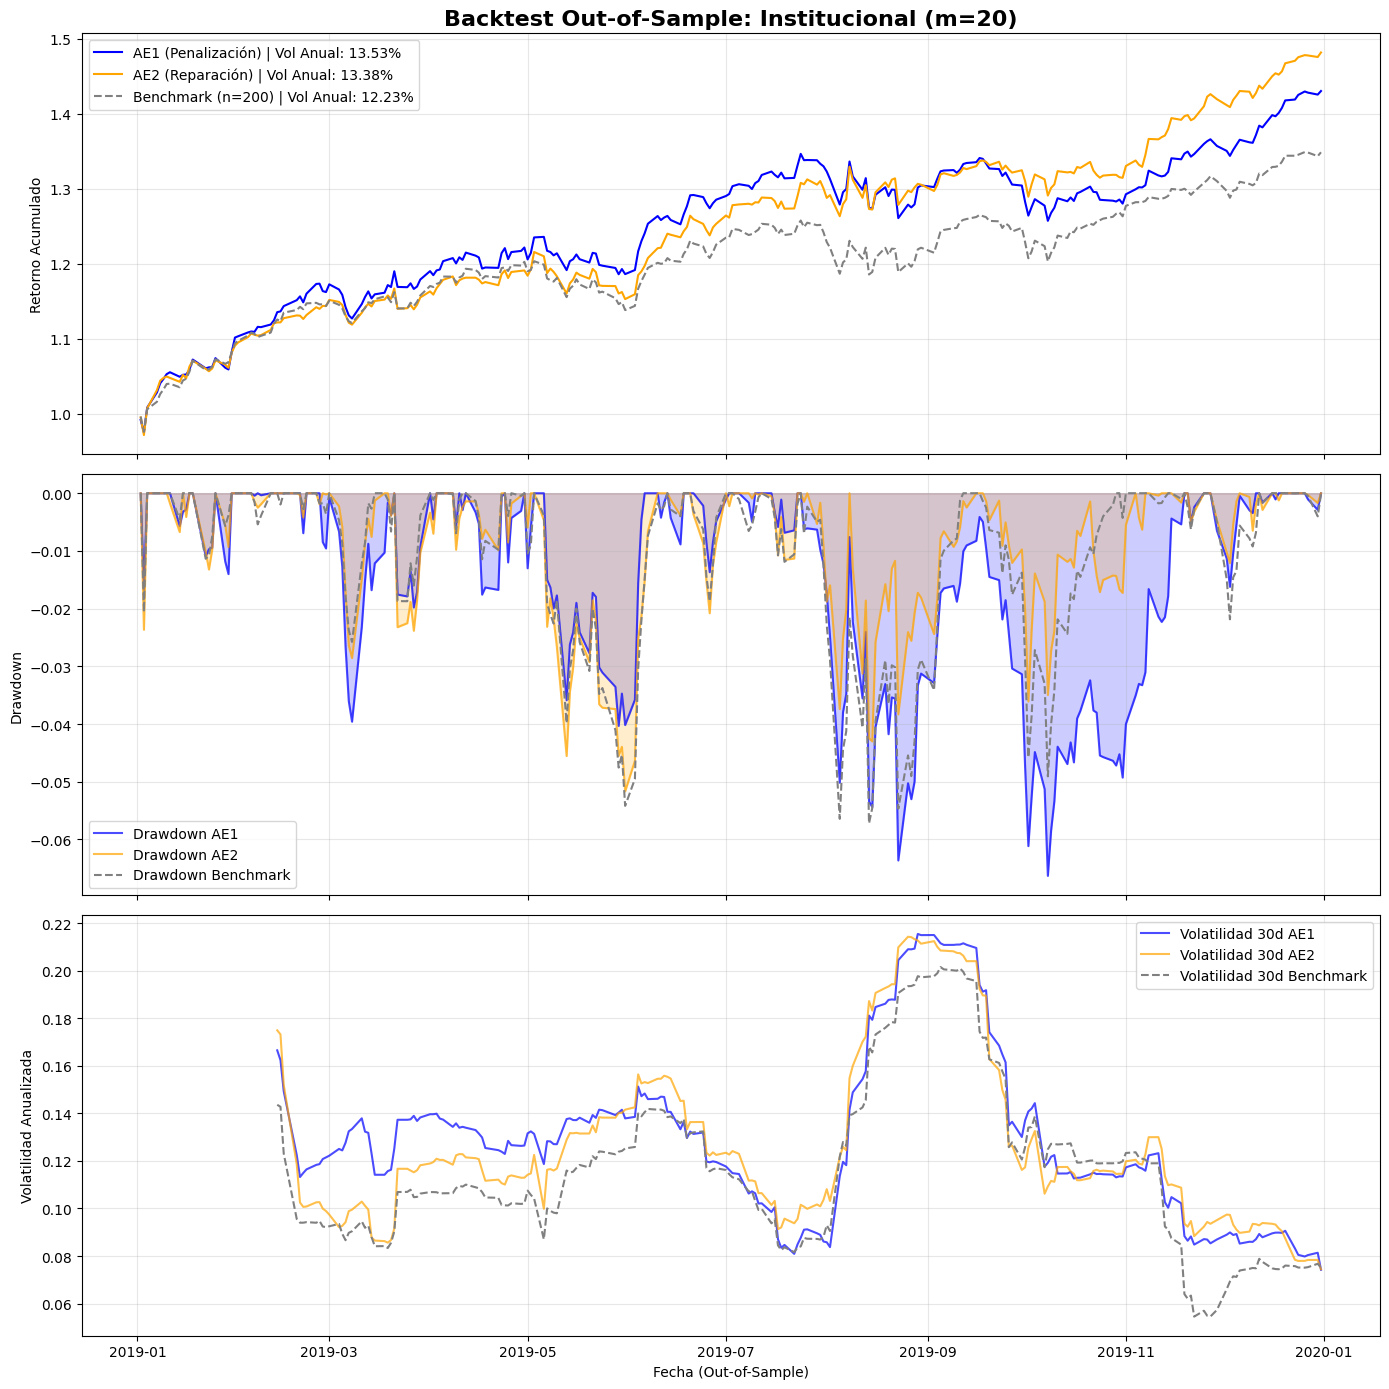
\includegraphics[width=\linewidth]{img/corr_backtest_institucional.png}
    \end{column}
  \end{columns}
\end{frame}

% --- Conclusiones P1 -------------------------------------
\begin{frame}{Conclusiones - Parte 1}
  \begin{columns}[T]
    \begin{column}{0.48\textwidth}
      \textbf{Hallazgos algorítmicos}
      \begin{enumerate}
        \item La \alert{reparación} supera a la \alert{penalización}
              en calidad de solución, confirmado estadísticamente
              en los 3 escenarios ($p=0{,}0020$).
        \item AE2 converge además con varianza mínima entre runs:
              es más robusto y reproducible.
      \end{enumerate}
    \end{column}
    \begin{column}{0.48\textwidth}
      \textbf{Hallazgos financieros}
      \begin{enumerate}
        \item Maximizar descorrelación \emph{no} implica minimizar
              el riesgo: ambas carteras optimizadas son \alert{más
              volátiles} que el benchmark amplio.
        \item Reducir a $m$ activos anula la diversificación por
              número de posiciones y eleva el riesgo idiosincrático.
        \item No hay diferencia sistemática AE1 vs AE2 en el
              backtest: lo domina la concentración de la cartera.
      \end{enumerate}
    \end{column}
  \end{columns}
\end{frame}

% =========================================================
%  PARTE 2
% =========================================================
\section{Parte 2 - Optimización con PSO (PySwarms)}

% --- Introducción PSO ------------------------------------
\begin{frame}{Introducción a PSO y Adaptación al Problema}
  \begin{columns}[T]
    \begin{column}{0.5\textwidth}
      \textbf{Particle Swarm Optimization (PSO)}
      \begin{itemize}
        \item Algoritmo bioinspirado basado en el movimiento de
              bandadas y bancos de peces.
        \item Cada \textbf{partícula} = solución candidata
              con posición y velocidad.
        \item Atracción hacia $\mathbf{p}_{\text{best}}$ (mejor
              personal) y $\mathbf{g}_{\text{best}}$ (mejor global).
      \end{itemize}

      \[
        v \leftarrow w\,v + c_1 r_1(\mathbf{p} - x) + c_2 r_2(\mathbf{g} - x)
      \]
    \end{column}
    \begin{column}{0.47\textwidth}
      \textbf{Dos aplicaciones en este trabajo}

      \begin{block}{Sección 1 - PSO Continuo}
        Optimizar los hiperparámetros $(p, d, q)$ del modelo
        ARIMA para predecir retornos semanales del SPY.
      \end{block}

      \vspace{8pt}
      \begin{block}{Sección 2 - PSO Binario}
        Selección de acciones del S\&P 500 como \emph{features}
        para predecir la dirección semanal del SPY
        (\emph{Wrapper Feature Selection}).
      \end{block}

      \vspace{6pt}
      \textbf{Librería:} \texttt{pyswarms}
    \end{column}
  \end{columns}
\end{frame}

% --- ARIMA -----------------------------------------------
\begin{frame}{Sección 1 - ARIMA y Función de Fitness}
  \begin{columns}[T]
    \begin{column}{0.5\textwidth}
      \textbf{El modelo ARIMA$(p,d,q)$}
      \begin{itemize}
        \item $p$: orden autorregresivo (cuántos valores pasados).
        \item $d$: grado de diferenciación (estacionariedad).
        \item $q$: orden de media móvil (errores pasados).
      \end{itemize}
      \textbf{Datos:} retornos \% semanales del SPY (2014-2025),
      descargados con \texttt{interval=``1wk''}.

      \vspace{8pt}
      \textbf{Función de fitness de cada partícula $(p,d,q)$}
      \[
        f = \underbrace{\text{RMSE}}_{\text{precisión}}
          + \underbrace{(1{,}5 - \text{DA})}_{\text{dirección}}
          + \underbrace{0{,}05(p+q)}_{\text{complejidad}}
      \]
      DA = fracción de predicciones con signo correcto.
    \end{column}
    \begin{column}{0.47\textwidth}
      \begin{block}{Esquema de rolling window}
        \vspace{4pt}
        \begin{tikzpicture}[scale=0.72]
          \draw[->] (0,0) -- (8,0) node[right]{\scriptsize Tiempo};
          \fill[primaryblue!30] (0,0.3) rectangle (4,0.8);
          \node[primaryblue, font=\scriptsize] at (2,0.55) {Train (208 sem.)};
          \fill[accentorange!30] (4,0.3) rectangle (5.2,0.8);
          \node[accentorange, font=\scriptsize] at (4.6,0.55) {Val (4)};
          \fill[green!30] (5.2,0.3) rectangle (5.7,0.8);
          \node[green!60!black, font=\scriptsize] at (5.45,0.55) {P};
          \draw[->, dashed, gray] (5.7,0.55) -- (6.5,0.55);
          \fill[primaryblue!30] (0.5,1.1) rectangle (4.5,1.6);
          \fill[accentorange!30] (4.5,1.1) rectangle (5.7,1.6);
          \fill[green!30] (5.7,1.1) rectangle (6.2,1.6);
        \end{tikzpicture}
      \end{block}

      \vspace{6pt}
      \begin{alertblock}{Ejecución cada 4 semanas}
        PSO re-optimiza $(p,d,q)$ mensualmente.
        Los parámetros se reusan las 4 semanas siguientes,
        reduciendo el coste computacional en $4\times$.
      \end{alertblock}
    \end{column}
  \end{columns}
\end{frame}

% --- Estrategias de trading ------------------------------
\begin{frame}{Sección 1 - Estrategias de Trading}
  \begin{columns}[T]
    \begin{column}{0.42\textwidth}
      \begin{block}{Comprar y Mantener (Benchmark)}
        $r_t = r_t^{\text{real}}$ \quad (posición larga fija)
      \end{block}
      \vspace{4pt}
      \begin{block}{Largo/Corto Base}
        $r_t = \text{sign}(\hat{r}_t) \cdot r_t^{\text{real}}$\\
        Opera ante cualquier señal, incluso débil.
      \end{block}
      \vspace{4pt}
      \begin{block}{L/C con Filtro ($>0{,}1\%$)}
        $r_t = \text{pos}_t \cdot r_t^{\text{real}}$\\
        Liquidez si $|\hat{r}_t| < \text{umbral}$.
        Filtra el ruido del mercado.
      \end{block}
      \vspace{4pt}
      \begin{block}{Solo Largo (Long Only)}
        $r_t = \mathbf{1}[\hat{r}_t>0] \cdot r_t^{\text{real}}$\\
        Liquidez si predicción negativa.
      \end{block}
    \end{column}
    \begin{column}{0.56\textwidth}
      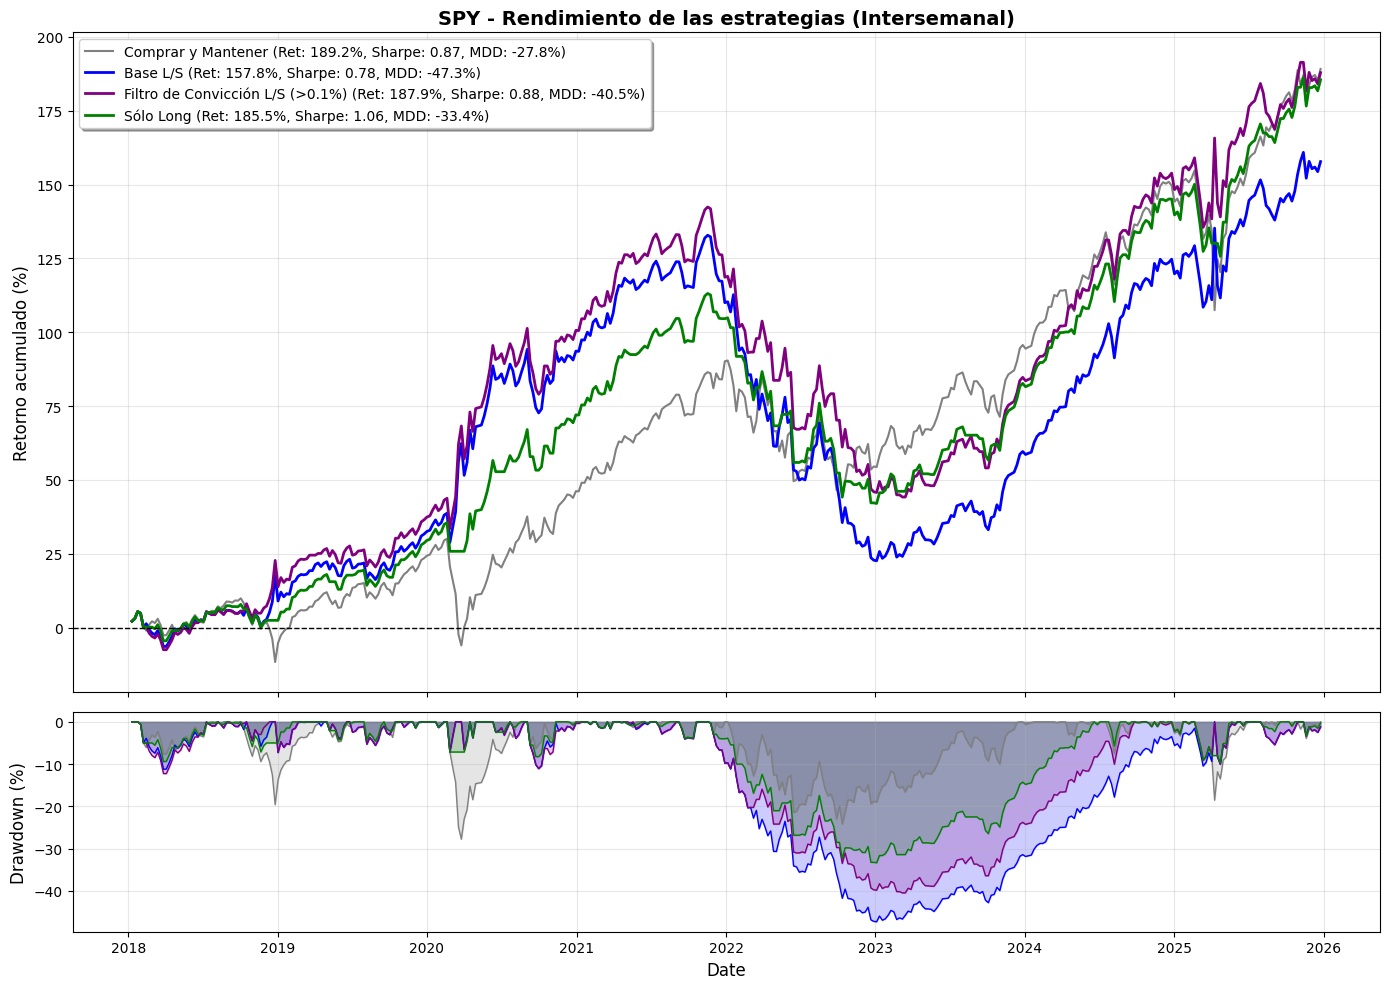
\includegraphics[width=\linewidth]{img/pso_estrategias.png}
    \end{column}
  \end{columns}
\end{frame}

% --- Análisis resultados trading -------------------------
\begin{frame}{Sección 1 - Análisis de Resultados}
  \begin{columns}[T]
    \begin{column}{0.5\textwidth}
      \textbf{Observaciones principales}
      \begin{itemize}
        \item Las estrategias activas superan al benchmark
              en retorno hasta mediados de 2022.
        \item \alert{2022: alta volatilidad} (inflación,
              tipos, guerra en Ucrania). El ARIMA lineal
              no captura cambios de régimen.
        \item \textbf{Solo Largo} es el más robusto a partir
              de 2022: evita pérdidas por posiciones cortas
              en mercados alcistas.
        \item L/C Base acumula los mayores drawdowns en
              periodos de incertidumbre.
      \end{itemize}
      
    \end{column}
    \begin{column}{0.48\textwidth}
      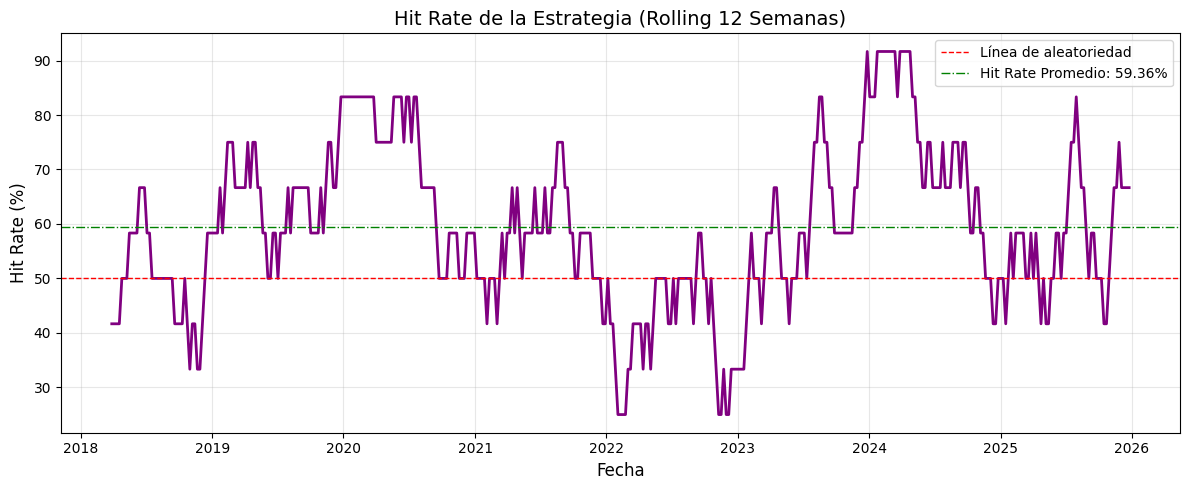
\includegraphics[width=\linewidth]{img/pso_hit_rate.png}

      \vspace{4pt}
      {\small Hit Rate rolling 12 semanas. Media $>50\%$ (supera
      la aleatoriedad). Picos $>90\%$ en mercados estables;
      caída pronunciada en 2022.}
      \begin{alertblock}{Limitación de ARIMA}
        Los mercados son no lineales; ARIMA captura
        patrones históricos pero no heteroscedasticidad
        ni cambios de régimen.
      \end{alertblock}
    \end{column}
  \end{columns}
\end{frame}

% --- Matriz de predicciones ------------------------------
\begin{frame}{Sección 1 - Predicciones vs.\ Realidad}
  \begin{columns}[T]
    \begin{column}{0.42\textwidth}
      \textbf{Lectura del diagrama de dispersión}
      \begin{itemize}
        \item \textcolor{green!60!black}{\textbf{Verde}}: predicción y
              retorno real tienen el mismo signo (acierto).
        \item \textcolor{red}{\textbf{Rojo}}: signos opuestos (error).
        \item Cuadrante I (++): aciertos Long.
        \item Cuadrante III (--): aciertos Short.
        \item Cuadrantes II y IV: errores.
      \end{itemize}

      \vspace{8pt}
      \textbf{Conclusión}\\
      La nube de puntos verdes supera a la de rojos,
      confirmando que el modelo ARIMA+PSO captura
      la dirección del mercado mejor que el azar.
    \end{column}
    \begin{column}{0.56\textwidth}
      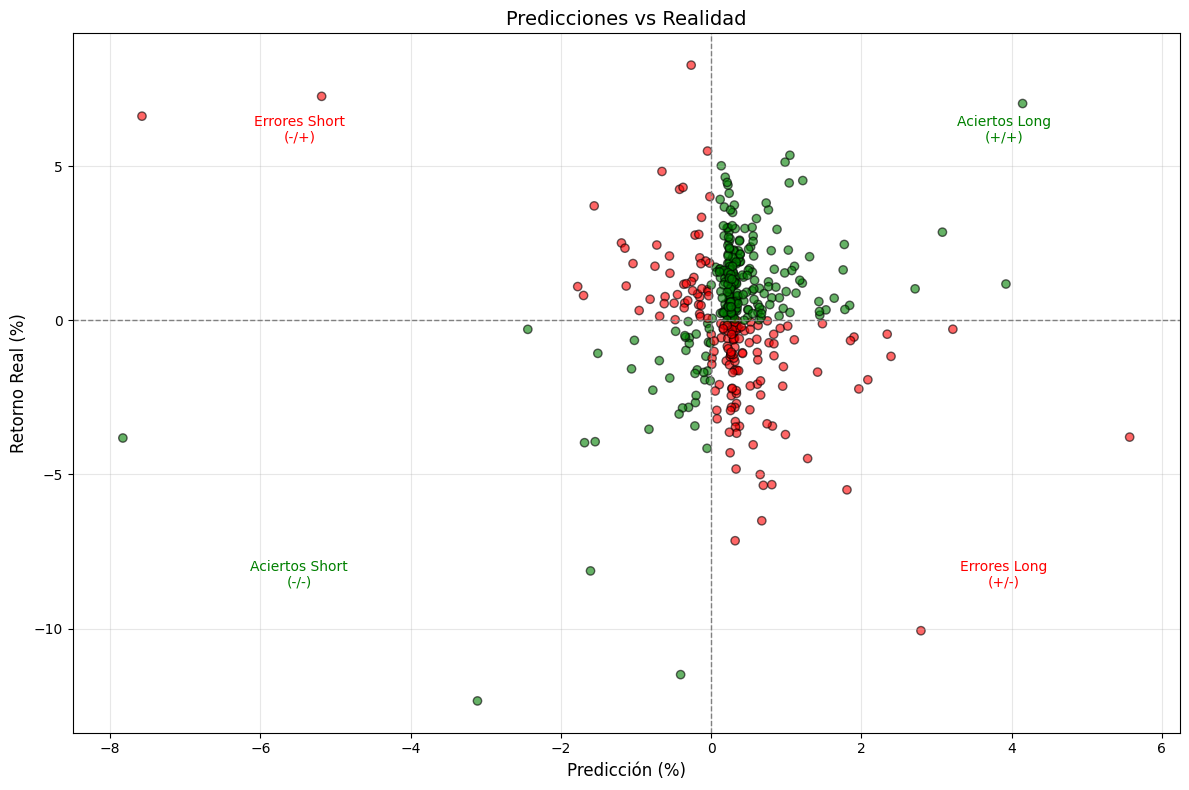
\includegraphics[width=\linewidth]{img/pso_pred_matrix.png}
    \end{column}
  \end{columns}
\end{frame}

% --- Evolución parámetros ARIMA -------------------------
\begin{frame}{Sección 1 - Evolución de los Parámetros ARIMA}
  \begin{columns}[T]
    \begin{column}{0.45\textwidth}
      \textbf{¿Qué muestra esta gráfica?}
      \begin{itemize}
        \item Evolución temporal de los parámetros $(p, d, q)$
              seleccionados por PSO a lo largo de los años.
        \item Cada escalón = PSO encontró parámetros
              distintos a los de la semana anterior.
        \item El parámetro $d$ (diferenciación) tiende
              a estabilizarse en 0 o 1, ya que los
              retornos son aproximadamente estacionarios.
        \item Los parámetros $p$ y $q$ cambian con más
              frecuencia, reflejando la adaptación del
              modelo a distintos regímenes de mercado.
      \end{itemize}
    \end{column}
    \begin{column}{0.55\textwidth}
      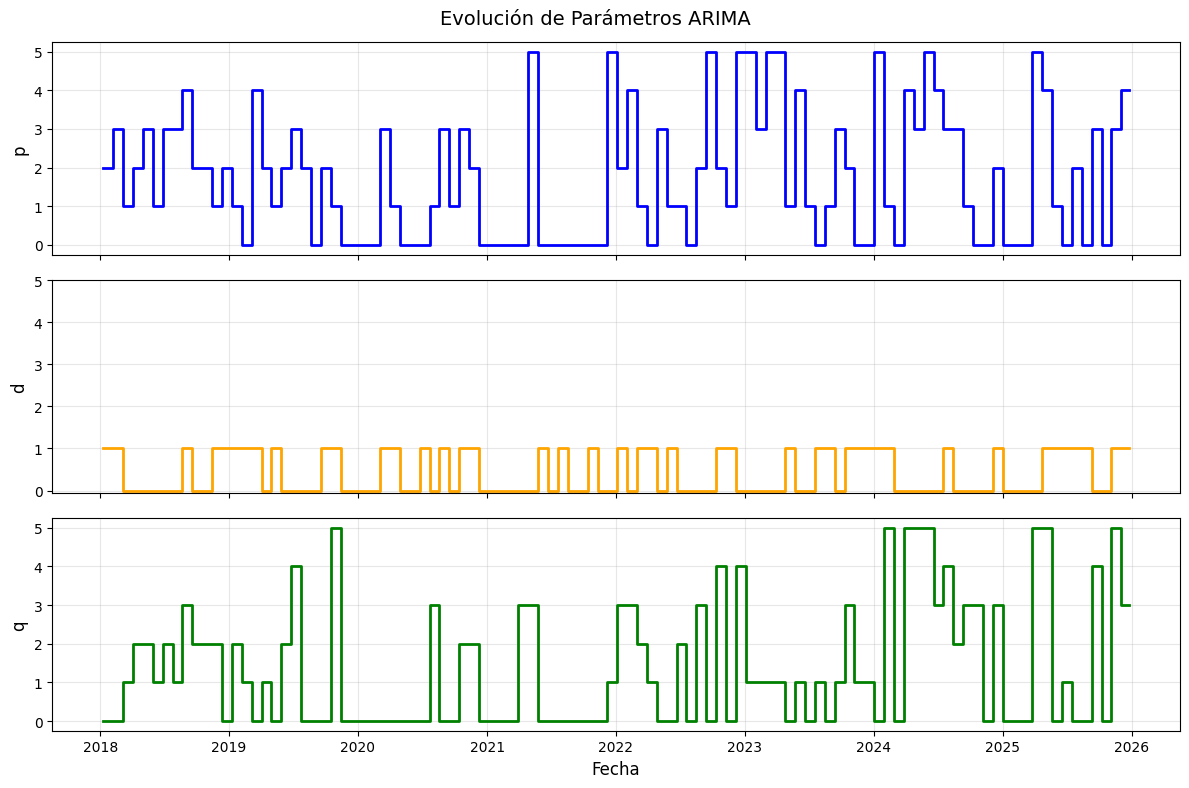
\includegraphics[width=\linewidth]{img/pso_params_arima.png}
    \end{column}
  \end{columns}
\end{frame}

% --- Evolución coste PSO ---------------------------------
\begin{frame}{Sección 1 - Coste PSO a lo Largo del Tiempo}
  \begin{columns}[T]
    \begin{column}{0.36\textwidth}
      \textbf{Interpretación del coste}
      \begin{itemize}
        \item Coste PSO bajo $\Rightarrow$ el modelo ARIMA
              se ajusta bien a ese periodo: mercado predecible.
        \item Coste PSO alto $\Rightarrow$ mercado difícil
              (2020 COVID, 2022 inflación).
        \item El \emph{warm start} (partir de los parámetros
              anteriores) acelera la convergencia.
        \item El delta de coste (panel inferior) muestra
              la magnitud del ajuste entre semanas.
      \end{itemize}
    \end{column}
    \begin{column}{0.62\textwidth}
      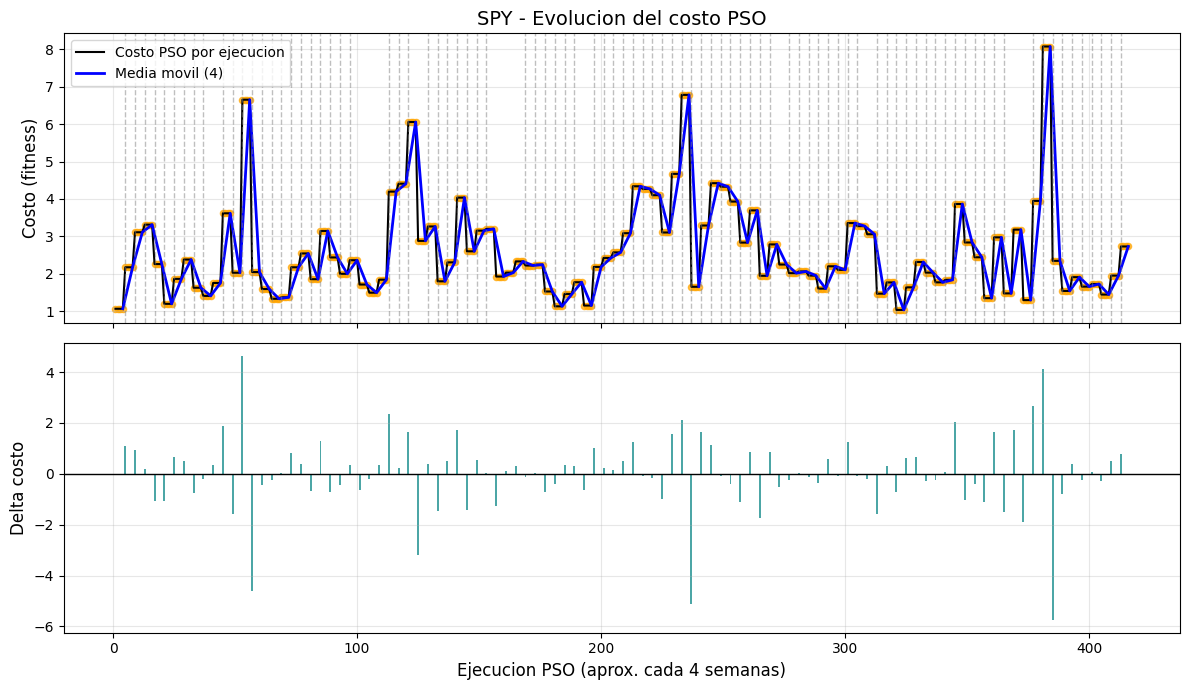
\includegraphics[width=\linewidth]{img/pso_cost_history.png}
    \end{column}
  \end{columns}
\end{frame}

% --- Binary PSO ------------------------------------------
\begin{frame}{Sección 2 - PSO Binario: Wrapper Feature Selection}
  \begin{columns}[T]
    \begin{column}{0.52\textwidth}
      \textbf{Reformulación del problema}
      \begin{itemize}
        \item \textbf{Features candidatas:} 25 acciones
              representativas del S\&P 500.
        \item \textbf{Target:} dirección semanal del SPY
              ($y_t = 1$ si sube, $0$ si baja).
        \item \textbf{Partícula:} máscara binaria de 25 bits.
        \item \textbf{Fitness:} $1 - \text{BAcc}$ del Random Forest
              en validación (a minimizar).
      \end{itemize}

      \vspace{6pt}
      \textbf{División temporal}
      \begin{itemize}
        \item Train PSO: 2014-2017 (208 semanas)
        \item Val PSO: 2018 (52 semanas)
        \item Test OOS: 2019 (51 semanas)
      \end{itemize}
    \end{column}
    \begin{column}{0.45\textwidth}
      \begin{block}{Configuración BinaryPSO}
        \begin{itemize}
          \item 25 dimensiones (una por acción).
          \item $w=0{,}7$, $c_1=c_2=1{,}4$.
          \item Topología \emph{fully connected}.
          \item 10 partículas, 30 iteraciones.
          \item 10 ejecuciones independientes.
        \end{itemize}
      \end{block}

      \vspace{6pt}
      \begin{block}{¿Por qué Balanced Accuracy?}
        La distribución de clases no es balanceada
        (más semanas alcistas).
        BAcc corrige este sesgo y penaliza clasificadores
        que ignoran la clase minoritaria.
      \end{block}
    \end{column}
  \end{columns}
\end{frame}

% --- Convergencia WFS ------------------------------------
\begin{frame}{Sección 2 - Convergencia del PSO Binario}
  \begin{columns}[T]
    \begin{column}{0.38\textwidth}
      \textbf{Evolución del coste (10 runs)}
      \begin{itemize}
        \item Líneas tenues = runs individuales.
        \item Línea gruesa azul = media de los 10 runs.
        \item La media desciende por debajo de la
              \emph{línea de aleatoriedad} ($\text{BAcc}=0.5$)
              desde las primeras iteraciones.
        \item La dispersión entre runs se reduce:
              el enjambre converge.
        \item A partir de la iteración 15, las mejoras
              son marginales.
      \end{itemize}

      \vspace{6pt}
     
    \end{column}
    \begin{column}{0.60\textwidth}
      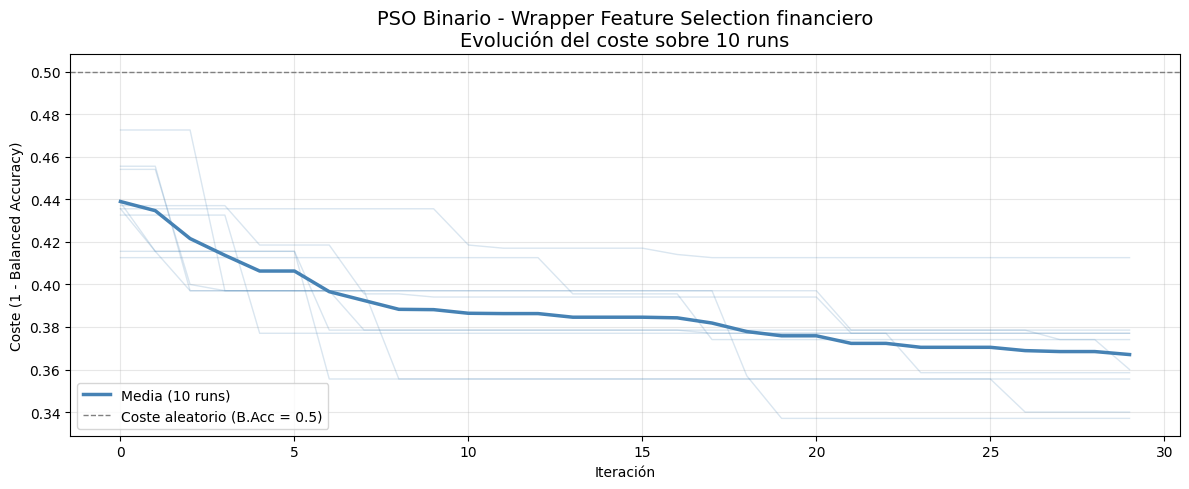
\includegraphics[width=\linewidth]{img/pso_wfs_convergencia.png}
       \begin{block}{Espacio de búsqueda}
        $2^{25} \approx 33\text{M}$ subconjuntos.
        Solo 300 evaluaciones. El PSO
        supera el azar sistemáticamente.
      \end{block}
    \end{column}
  \end{columns}
\end{frame}

% --- Heatmap selección -----------------------------------
\begin{frame}{Sección 2 - Patrón de Selección de Acciones}
  \begin{columns}[T]
    \begin{column}{0.45\textwidth}
      \textbf{Lecturas del heatmap y barras}
      \begin{itemize}
        \item \textbf{MSFT, GOOGL} (8/10 runs): sector
              tecnológico de gran capitalización contiene
              más información predictiva sobre el SPY.
        \item \textbf{PFE, WMT, JNJ, PG\ldots} (6-7/10):
              acciones defensivas también relevantes.
        \item \textbf{ABT, HD} (1-2/10): baja contribución
              marginal a la predicción del índice.
        \item La cardinalidad varía entre 6 y 18 acciones:
              el PSO no impone ninguna restricción al respecto.
      \end{itemize}
    \end{column}
    \begin{column}{0.55\textwidth}
      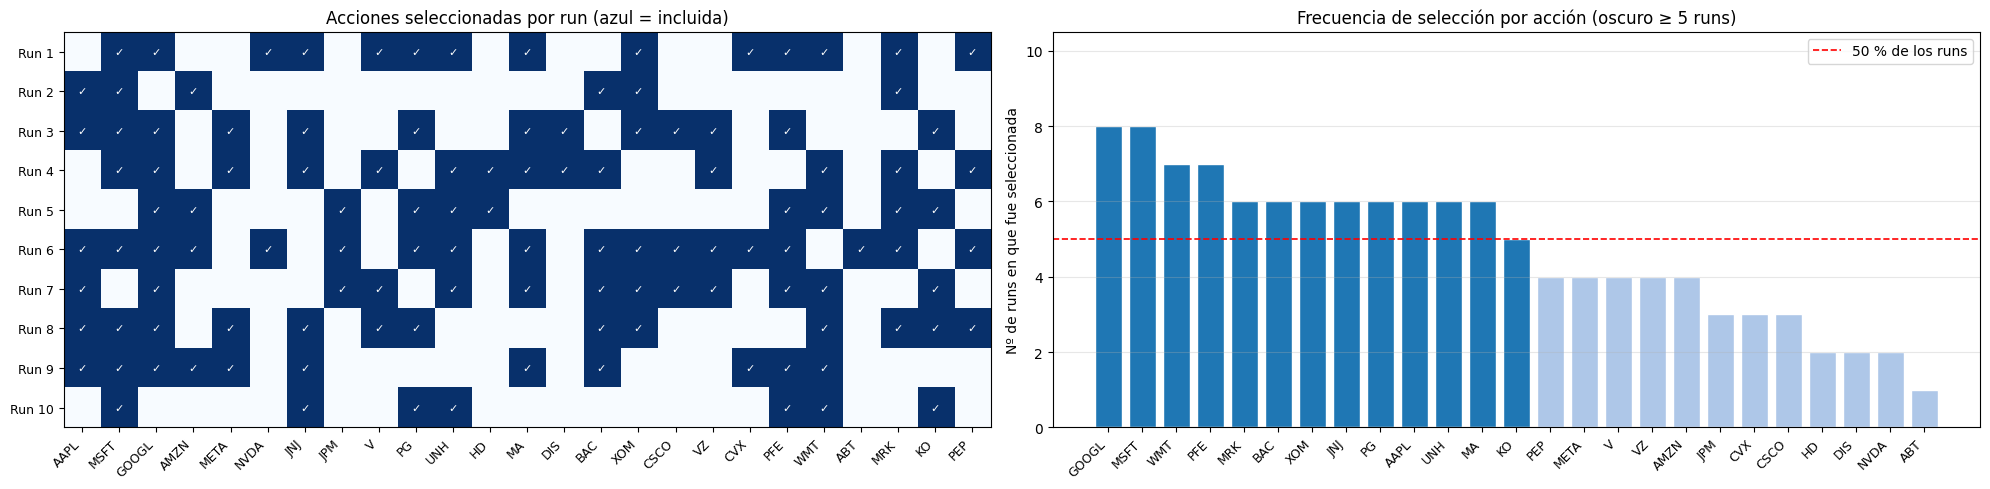
\includegraphics[width=\linewidth,clip=true,trim=0 0 715 0]{img/pso_wfs_heatmap.png}
    \end{column}
  \end{columns}
\end{frame}

% --- Sobreajuste -----------------------------------------
\begin{frame}{Sección 2 - Sobreajuste y Balanced Accuracy}
  \begin{columns}[T]
    \begin{column}{0.36\textwidth}
      \textbf{Resultados (10 runs)}
      \begin{itemize}
        \item BAcc Train = 1.0 en \emph{todos} los runs:
              el Random Forest memoriza perfectamente
              los 208 patrones de entrenamiento.
        \item BAcc Test promedio $\approx 0.571$, con el
              mejor run llegando a $0.653$.
        \item Todos superan la barrera del $0.5$
              (clasificador aleatorio), lo que indica
              capacidad predictiva genuina.
        \item La brecha media Train-Test es $0.43$:
              sobreajuste sistematico, pero no inutilizante.
      \end{itemize}
    \end{column}
    \begin{column}{0.62\textwidth}
      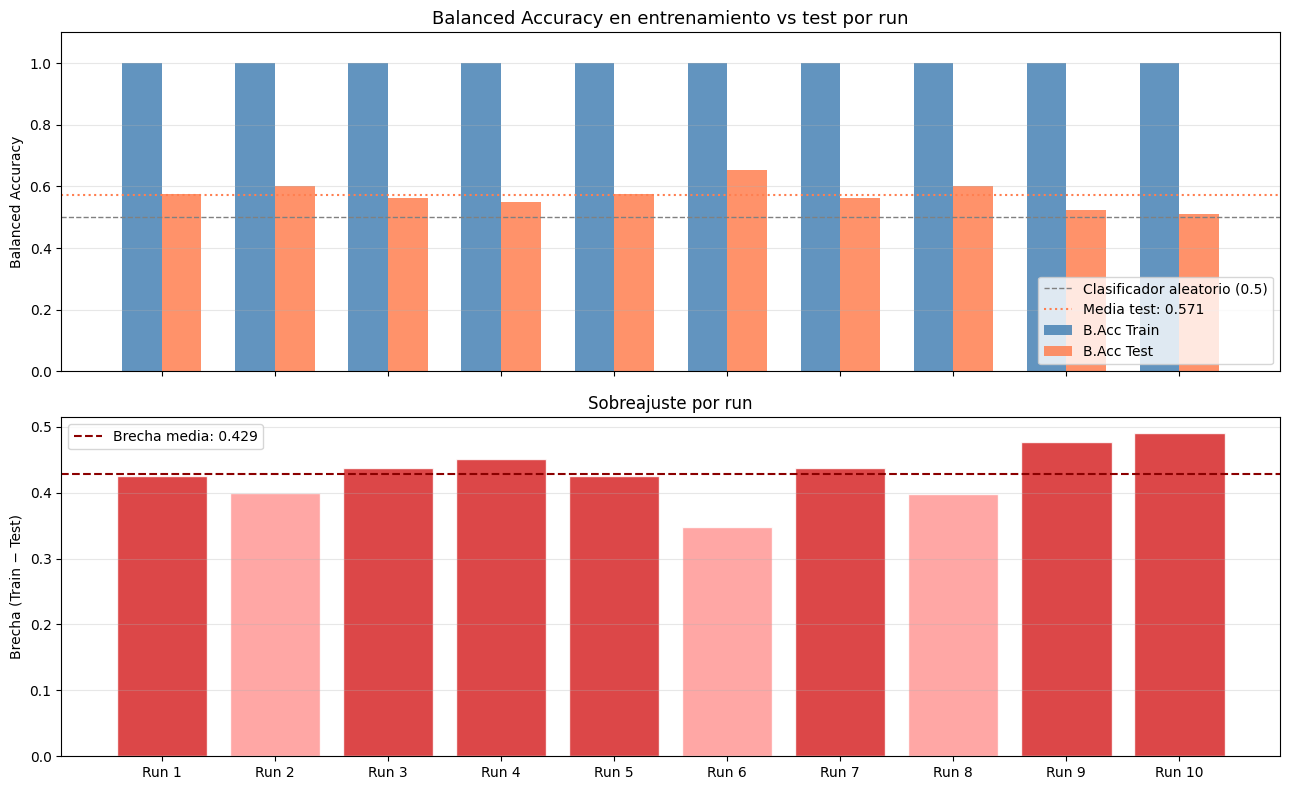
\includegraphics[width=\linewidth]{img/pso_wfs_overfitting.png}
    \end{column}
  \end{columns}
\end{frame}

% --- Comparativa PSO1 vs PSO2 ----------------------------
\begin{frame}{Comparativa: PSO Continuo vs.\ PSO Binario}
  \begin{columns}[T]
    \begin{column}{0.48\textwidth}
      \begin{block}{PSO Continuo (Sección 1)}
        \begin{tabular}{ll}
          \textbf{Espacio} & $\mathbb{N}^3$, continuo* \\
          \textbf{Dimensiones} & 3 ($p, d, q$) \\
          \textbf{Evaluación} & Ajuste ARIMA + RMSE \\
          \textbf{Coste eval.} & Alto (modelo ARIMA) \\
          \textbf{Resultado} & Parámetros temporales \\
        \end{tabular}
      \end{block}
    \end{column}
    \begin{column}{0.48\textwidth}
      \begin{block}{PSO Binario (Sección 2)}
        \begin{tabular}{ll}
          \textbf{Espacio} & $\{0,1\}^{25}$, discreto \\
          \textbf{Dimensiones} & 25 (una por acción) \\
          \textbf{Evaluación} & Random Forest + BAcc \\
          \textbf{Coste eval.} & Moderado (RF estático) \\
          \textbf{Resultado} & Subconjunto de features \\
        \end{tabular}
      \end{block}
    \end{column}
  \end{columns}
  \begin{alertblock}{Conclusión comparativa}
    PSO continuo: adecuado para ajustar modelos adaptativos con pocos parámetros
    pero evaluaciones costosas.
    PSO binario: adecuado para selección de variables en espacios combinatorios
    donde la búsqueda exhaustiva es inviable.
    Ambos usos son complementarios y cubren necesidades distintas del análisis financiero.
  \end{alertblock}
\end{frame}

% --- Conclusiones P2 --------------------------------------
\begin{frame}{Conclusiones - Parte 2}
  \begin{columns}[T]
    \begin{column}{0.48\textwidth}
      \textbf{PSO Continuo para ARIMA}
      \begin{enumerate}
        \item El PSO adaptativo mejora la selección de
              parámetros frente a una búsqueda fija.
        \item La estrategia \textbf{Solo Largo} es la más
              robusta ante shocks de mercado.
        \item El filtro de convicción reduce señales
              débiles, mejorando el Sharpe.
        \item ARIMA tiene limitaciones ante cambios de
              régimen (no linealidad del mercado).
      \end{enumerate}
    \end{column}
    \begin{column}{0.48\textwidth}
      \textbf{PSO Binario para Feature Selection}
      \begin{enumerate}
        \item PSO identifica subconjuntos con capacidad
              predictiva real sobre el SPY.
        \item El sobreajuste con Random Forest es inevitable
              en ventanas históricas cortas.
        \item MSFT y GOOGL son los predictores más robustos
              en los 10 runs.
        \item La composición del subconjunto importa más
              que su cardinalidad.
      \end{enumerate}
    \end{column}
  \end{columns}

  \vspace{8pt}
  % \begin{block}{Trabajos futuros}
  %   \small
  %   \begin{itemize}
  %     \item Sustituir ARIMA por modelos no lineales (LSTM, XGBoost) en Sección 1.
  %     \item Añadir restricciones de cardinalidad al PSO binario.
  %     \item Combinar ambas partes: usar el subconjunto de Sección 2 como
  %           input del modelo predictivo de la Sección 1.
  %   \end{itemize}
  % \end{block}
\end{frame}

% --- Diapositiva final -----------------------------------
\begin{frame}[plain]
  \vfill
  \begin{center}
    {\Large \textbf{¿Preguntas?}}

    \vspace{20pt}
    {\normalsize
      \begin{tabular}{rl}
        Parte 1: & Máxima Diversidad con AE1 (Penalización) y AE2 (Reparación) \\
        Parte 2: & PSO Continuo para ARIMA y PSO Binario para Feature Selection \\
      \end{tabular}
    }

    \vspace{20pt}
    {\small
      Datos: Yahoo Finance. S\&P 500. 2014-2025 \\
      Herramientas: \texttt{yfinance}, \texttt{pyswarms}, \texttt{statsmodels},
      \texttt{scikit-learn}, \texttt{scipy}
    }
  \end{center}
  \vfill
\end{frame}

\end{document}
